\section*{(21\textordfeminine\ aula) --- Momento Angular e Rotações}

\subsection*{Momento Angular e Rotações}

Agora que conhecemos melhor os operadores $\hat{L}_x, \hat{L}_y, \hat{L}_z$ e $\hat{L}^2$, vamos mostrar como eles estão relacionados a rotações. Vamos seguir a mesma linha usada para mostrar que o operador de translação é

\begin{equation}
    \fbox{estudar} \longrightarrow T(\vec{a}) = \exp\left[-i\,\vec{P}\cdot\vec{a}/\hbar\right]
\label{eq:aula21_T_def}
\end{equation}
(nova notação para operadores)

Recapitulando (agora para o espaço vetorial de estados de uma partícula em 3D) o que vimos na 1\textsuperscript{a} aula.

\textbf{1) Definição:}
\begin{equation}
    \bra{\vec{r}} T(\vec{a}) \ket{\Psi} = \Psi(\vec{r} - \vec{a})
\label{eq:aula21_T_def_acao}
\end{equation}

(a função de onda do estado transladado é $\Psi(\vec{r})$ rigidamente deslocada de $\vec{a}$).

\textbf{2) Considerando uma translação infinitesimal na direção $\hat{n}$}

\begin{equation}
    T(\vec{\varepsilon}) = \mathbb{I} + G\varepsilon + \Theta(\varepsilon^2) \qquad \text{($G$ desconhecido)}
\label{eq:aula21_T_infinitesimal}
\end{equation}

\begin{equation}
    \bra{\vec{r}} \mathbb{I} + G\varepsilon + \Theta(\varepsilon^2) \ket{\Psi} = \underbrace{\Psi(\vec{r}) - \varepsilon\,\hat{n}\cdot\vec{\nabla}\Psi + \Theta(\varepsilon^2)}_{\Psi(\vec{r}-\vec{\varepsilon})}
\label{eq:aula21_T_infinitesimal_acao}
\end{equation}

\begin{equation}
    \Longrightarrow \quad \bra{\vec{r}} G \ket{\Psi} = -\hat{n}\cdot\vec{\nabla}\Psi.
\label{eq:aula21_G_acao}
\end{equation}
Comparando com
\begin{equation}
    \bra{\vec{r}} \vec{P}\cdot\hat{n} \ket{\Psi} = -i\hbar\,\hat{n}\cdot\vec{\nabla}\Psi
\label{eq:aula21_P_acao}
\end{equation}
concluímos que
\begin{equation}
    \boxed{G = \frac{-i\,\vec{P}\cdot\hat{n}}{\hbar}}
\label{eq:aula21_G_resultado}
\end{equation}

\textbf{3) Uma translação finita nessa direção $\hat{n}$ é}
\begin{equation}
    \lim_{N\to\infty}\left[T\left(\frac{\vec{a}}{N}\right)\right]^N = \lim_{N\to\infty}\left[\mathbb{I} - i\frac{\vec{P}\cdot\hat{n}}{\hbar}\frac{a}{N}\right]^N
\label{eq:aula21_T_finita_limite}
\end{equation}

\begin{equation}
    \boxed{T(\vec{a}) = \exp\left[\frac{-i\,\vec{P}\cdot\vec{a}}{\hbar}\right]} \qquad \text{c.q.d.}
\label{eq:aula21_T_finita_resultado}
\end{equation}

\subsection*{O que significa "rotacionar" em MQ}

Para começar, precisamos saber o que se quer dizer com "rotação". Em MQ, "rotacionar" o estado $(\vec{r}, \vec{p})$ de $\theta$ em torno da direção $\hat{n}$ significa:

\begin{center}
\begin{tikzpicture}[scale=1.1]
    \draw[->] (0,0) -- (0,3.2) node[above] {$z$};
    \draw[->] (0,0) -- (-1.8,-1) node[below left] {$x$};
    \draw[->] (0,0) -- (3.3,0) node[right] {$y$};
    \draw[->,thick] (0,0) -- (1.4,2.2) node[above] {$\hat{n}$};
    \draw[->,thick,dashed] (0,0) -- (2.0,1.3) node[right] {$\vec{r}$};
    \draw[->,thick,dashed] (0,0) -- (0.9,1.9) node[above left] {$\vec{r}\,'$};
    \draw[->,thick] (2.0,1.3) -- (2.9,2.0) node[right] {$\vec{p}$};
    \draw[->,thick] (0.9,1.9) -- (1.5,2.7) node[above] {$\vec{p}\,'$};
    \draw (1.3,1.0) arc (15:65:0.6);
    \node at (1.55,1.45) {\small $\theta$};
\end{tikzpicture}
\end{center}

De forma incremental da translação, o vetor $\vec{p}$ se modifica da mesma maneira que o vetor $\vec{r}$. A relação entre $\vec{r}$ e $\vec{r}\,'$ e $\vec{p}$ e $\vec{p}\,'$ se expressa por meio da chamada \textbf{MATRIZ DE ROTAÇÃO}

\begin{equation}
    \begin{bmatrix} x' \\ y' \\ z' \end{bmatrix}
    =
    R(\theta\hat{n})
    \begin{bmatrix} x \\ y \\ z \end{bmatrix}
\label{eq:aula21_matriz_rotacao}
\end{equation}
onde o vetor da esquerda tem componentes de $\vec{r}\,'$ e o vetor da direita tem componentes de $\vec{r}$.

Exatamente a mesma matriz relaciona $\vec{p}$ com $\vec{p}\,'$. Não vamos construir essa matriz pois, como vimos, apenas as propriedades da rotação \textbf{INFINITESIMAL} serão usadas. (No curso de Mecânica Clássica obtivemos essas matrizes.)

\subsection*{Rotação infinitesimal}

No caso de $\theta = \varepsilon$ ser um ângulo muito pequeno:

\begin{center}
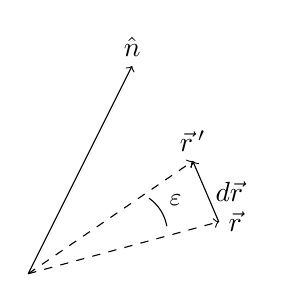
\begin{tikzpicture}[scale=1.1]
    \draw[->] (0,0) -- (1.2,2.4) node[above] {$\hat{n}$};
    \draw[->,dashed] (0,0) -- (2.2,0.6) node[right] {$\vec{r}$};
    \draw[->,dashed] (0,0) -- (1.9,1.3) node[above] {$\vec{r}\,'$};
    \draw[->] (2.2,0.6) -- (1.9,1.3) node[midway, right] {$d\vec{r}$};
    \draw (1.6,0.55) arc (10:55:0.5);
    \node at (1.7,0.85) {\small $\varepsilon$};
\end{tikzpicture}
\end{center}

\begin{equation}
    \vec{r}\,' = \vec{r} + d\vec{r} = \vec{r} + (\hat{n}\times\vec{r})\,\varepsilon + \Theta(\varepsilon^2)
\label{eq:aula21_r_linha}
\end{equation}
similarmente,
\begin{equation}
    \vec{p}\,' = \vec{p} + (\hat{n}\times\vec{p})\,\varepsilon + \Theta(\varepsilon^2).
\label{eq:aula21_p_linha}
\end{equation}

Agora a definição da ação do operador de rotação:

\begin{equation}
    \fbox{1)} \qquad \bra{\vec{r}} U(\theta,\hat{n}) \ket{\Psi} = \Psi(R^{-1}\vec{r})
\label{eq:aula21_U_def}
\end{equation}

ou seja, a função de onda do estado rodado deve ser $\Psi(\vec{r})$ rigidamente girada de $\theta$ na direção $\hat{n}$.

\begin{center}
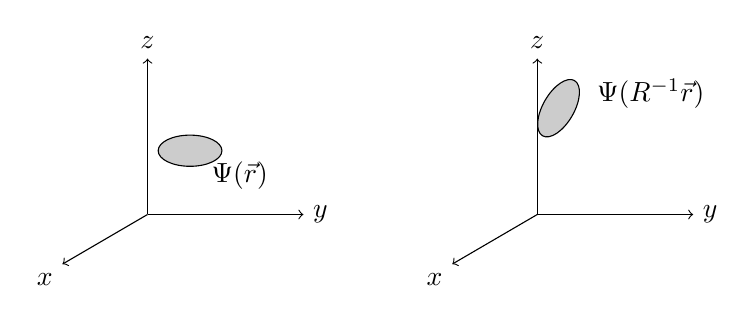
\begin{tikzpicture}[scale=0.9]
    \begin{scope}
        \draw[->] (0,0) -- (0,2.2) node[above] {$z$};
        \draw[->] (0,0) -- (-1.2,-0.7) node[below left] {$x$};
        \draw[->] (0,0) -- (2.2,0) node[right] {$y$};
        \draw[fill=gray!40] (0.6,0.9) ellipse (0.45 and 0.22);
        \node at (1.3,0.55) {$\Psi(\vec{r})$};
    \end{scope}
    \begin{scope}[xshift=5.5cm]
        \draw[->] (0,0) -- (0,2.2) node[above] {$z$};
        \draw[->] (0,0) -- (-1.2,-0.7) node[below left] {$x$};
        \draw[->] (0,0) -- (2.2,0) node[right] {$y$};
        \draw[fill=gray!40, rotate around={60:(0.3,1.5)}] (0.3,1.5) ellipse (0.45 and 0.22);
        \node at (1.6,1.7) {$\Psi(R^{-1}\vec{r})$};
    \end{scope}
\end{tikzpicture}
\end{center}

O valor da nova função de onda em $\vec{r}$ é igual ao valor da antiga em $R^{-1}\vec{r}$ ($R^{-1}$ representa a matriz de rotação inversa).

\begin{center}
\begin{tabular}{ll}
Função $\Psi(\vec{r})$ transladada de $\vec{a}$: & $\Psi(\vec{r}-\vec{a})$ \\
Função $\Psi(\vec{r})$ girada de $\theta$ na direção $\hat{n}$: & $\Psi\big(R(-\theta,\hat{n})\,\vec{r}\big)$
\end{tabular}
\end{center}

\textbf{2) Considerando uma rotação infinitesimal na direção $\hat{n}$}

\begin{equation}
    \bra{\vec{r}} \mathbb{I} + G\varepsilon + \Theta(\varepsilon^2) \ket{\Psi} = \Psi\big(\vec{r} - (\hat{n}\times\vec{r})\varepsilon + \Theta(\varepsilon^2)\big)
\label{eq:aula21_U_infinitesimal}
\end{equation}
onde o argumento da direita é a rotação infinitesimal de $\vec{r}$ no sentido contrário.

\begin{equation}
    = \Psi(\vec{r}) - (\hat{n}\times\vec{r})\,\varepsilon\cdot\vec{\nabla}\Psi + \Theta(\varepsilon^2)
\label{eq:aula21_U_infinitesimal_expandido}
\end{equation}

\begin{equation}
    \Longrightarrow \quad \bra{\vec{r}} G \ket{\Psi} = -(\hat{n}\times\vec{r})\cdot\vec{\nabla}\Psi = -\hat{n}\cdot(\vec{r}\times\vec{\nabla}\Psi)
\label{eq:aula21_G_rotacao}
\end{equation}

Comparando com
\begin{equation}
    \bra{\vec{r}} \vec{L}\cdot\hat{n} \ket{\Psi} = \hat{n}\cdot\bra{\vec{r}}\vec{L}\ket{\Psi} = -i\hbar\,\hat{n}\cdot(\vec{r}\times\vec{\nabla}\Psi)
\label{eq:aula21_L_acao}
\end{equation}

Concluímos que
\begin{equation}
    \boxed{G = \frac{-i}{\hbar}\,\vec{L}\cdot\hat{n}}
\label{eq:aula21_G_rotacao_resultado}
\end{equation}

\textbf{3) Uma rotação finita na direção $\hat{n}$ pode ser obtida com uma sequência de rotações infinitesimais}, unitárias como $T(\vec{a})$:

\begin{equation}
    \lim_{N\to\infty}\left[\mathbb{I} - i\,\frac{\vec{L}\cdot\hat{n}}{\hbar}\,\frac{\theta}{N}\right]^N = \exp\left[\frac{-i\,\vec{L}\cdot\hat{n}}{\hbar}\,\theta\right] \equiv U(\vec{\theta})
\label{eq:aula21_U_finita}
\end{equation}

Dizemos que $\vec{P}\cdot\hat{n}$ é o gerador das translações na direção $\hat{n}$, assim como $\dfrac{\vec{L}\cdot\hat{n}}{\hbar}$ é o gerador das rotações na direção $\hat{n}$.

\subsection*{Comentários}

\textbf{(i)} Escolhida a direção $\hat{n}$, tanto $\vec{P}\cdot\hat{n}$ quanto $\vec{L}\cdot\hat{n}$ são operadores perfeitamente bem definidos.

\textbf{Exemplo:} $\hat{n} = \dfrac{1}{\sqrt{2}}\hat{i} + \dfrac{1}{\sqrt{2}}\hat{j}$

\begin{equation}
    \hat{n}\cdot\vec{P} = \frac{\hat{P}_x}{\sqrt{2}} + \frac{\hat{P}_y}{\sqrt{2}}
    \qquad \text{e} \qquad
    \hat{n}\cdot\vec{L} = \frac{\hat{L}_x}{\sqrt{2}} + \frac{\hat{L}_y}{\sqrt{2}}
\label{eq:aula21_exemplo_n}
\end{equation}

\textbf{(ii)} Os operadores de translação comutam, pois os operadores $\vec{P}$ comutam. Isso não acontece com os operadores de rotação.

\textbf{Exemplo:}
\begin{equation}
    T(a\hat{i})\,T(b\hat{j}) = e^{-i\hat{P}_x a/\hbar}\,e^{-i\hat{P}_y b/\hbar} = T(b\hat{j})\,T(a\hat{i})
\label{eq:aula21_comutam_translacao}
\end{equation}

\begin{equation}
    U(\alpha\hat{i})\,U(\beta\hat{j}) = e^{-i\hat{L}_x\alpha/\hbar}\,e^{-i\hat{L}_y\beta/\hbar}
    \;\neq\;
    e^{-i\hat{L}_y\beta/\hbar}\,e^{-i\hat{L}_x\alpha/\hbar}
    = U(\beta\hat{j})\,U(\alpha\hat{i})
\label{eq:aula21_nao_comutam_rotacao}
\end{equation}

Isso, contudo, não é uma particularidade de \textbf{TRANSLAÇÕES e ROTAÇÕES} na MQ. Lembre sempre que os operadores $T$ e $U$ agem sobre as funções de onda, transladando-as e rotacionando-as, como se essas fossem um objeto 3D qualquer. De fato, qualquer objeto (não apenas funções de onda) pode ser transladado em qualquer ordem, mas não pode ser rotacionado em qualquer ordem.

\subsubsection*{Translações: a ordem não importa}

Considere um cubo sendo transladado por $T_x$ e depois $T_y$, ou na ordem inversa: o estado final é o mesmo (o cubo chega à mesma posição final, deslocado por $\vec{a} = a_x\hat{i} + a_y\hat{j}$).

\begin{center}
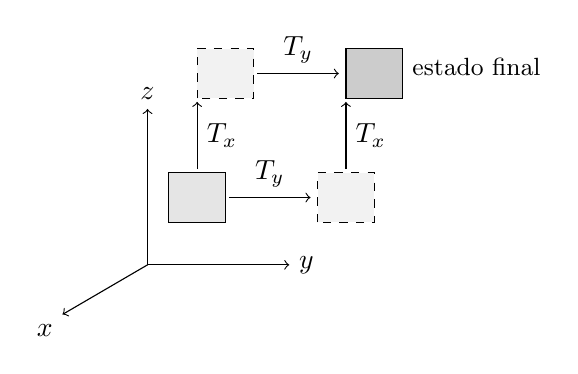
\begin{tikzpicture}[scale=0.9]
    \draw[->] (0,0) -- (0,2.2) node[above] {$z$};
    \draw[->] (0,0) -- (-1.2,-0.7) node[below left] {$x$};
    \draw[->] (0,0) -- (2,0) node[right] {$y$};
    \draw[fill=gray!20] (0.3,0.6) rectangle (1.1,1.3);
    \draw[->] (1.15,0.95) -- (2.3,0.95) node[midway,above] {$T_y$};
    \draw[->] (0.7,1.35) -- (0.7,2.3) node[midway,right] {$T_x$};
    \draw[dashed,fill=gray!10] (2.4,0.6) rectangle (3.2,1.3);
    \draw[->] (2.8,1.35) -- (2.8,2.3) node[midway,right] {$T_x$};
    \draw[dashed,fill=gray!10] (0.7,2.35) rectangle (1.5,3.05);
    \draw[->] (1.55,2.7) -- (2.7,2.7) node[midway,above] {$T_y$};
    \draw[fill=gray!40] (2.8,2.35) rectangle (3.6,3.05);
    \node[below right] at (3.6,3.05) {\small estado final};
\end{tikzpicture}
\end{center}

\subsubsection*{Rotações: a ordem importa}

Considere um dado (cubo com faces numeradas) sendo rotacionado por $R_y(\pi/2)$ seguido de $R_x(\pi/2)$ (sequência 1), e por $R_x(\pi/2)$ seguido de $R_y(\pi/2)$ (sequência 2). As orientações finais do dado são diferentes nos dois casos.

\textbf{(seq. 1):} $R_y(\pi/2)$ depois $R_x(\pi/2)$.

\textbf{(seq. 2):} $R_x(\pi/2)$ depois $R_y(\pi/2)$.

Observe que:
\begin{equation}
    \text{(seq. 1)} \qquad R_x(\pi/2)\,R_y(\pi/2) = R\left(\frac{2\pi}{3}, \frac{1}{\sqrt{3}}(\hat{i}+\hat{j}+\hat{k})\right)
\label{eq:aula21_seq1}
\end{equation}
onde o eixo $\dfrac{1}{\sqrt{3}}(\hat{i}+\hat{j}+\hat{k})$ é a diagonal do cubo, e o ângulo efetivo é $120^\circ$.

(É sempre possível escrever uma sequência de rotações como uma única rotação.) Você pode verificar também que:
\begin{equation}
    \text{(seq. 2)} \qquad R_y(\pi/2)\,R_x(\pi/2) = R\left(\frac{2\pi}{3}, \frac{1}{\sqrt{3}}(\hat{i}+\hat{j}-\hat{k})\right)
\label{eq:aula21_seq2}
\end{equation}

\textbf{(iii)} As operações de translação e de rotação são implementadas de maneiras diferentes na MC e na MQ, pois os "estados" são objetos matemáticos diferentes nos dois casos.

\begin{center}
\begin{tabular}{|l|c|c|}
\hline
 & Mec. Clássica & Mec. Quântica \\
\hline
transl.: & $(\vec{r},\vec{p}) \to (\vec{r}+\vec{a},\,\vec{p})$ & $\ket{\Psi} \to e^{-i\vec{P}\cdot\vec{a}/\hbar}\ket{\Psi}$ \\
\hline
rotação: & $(\vec{r},\vec{p}) \to (R\vec{r},\,R\vec{p})$ & $\ket{\Psi} \to e^{-i\vec{L}\cdot\hat{n}\,\theta/\hbar}\ket{\Psi}$ \\
\hline
\end{tabular}
\end{center}
onde $R$ (matriz $3\times 3$ de rotação) é a matriz de rotação $3\times 3$.

\subsection*{Invariância de Rotação}

Um problema com simetria de rotação em relação ao eixo $\hat{n}$ é caracterizado, na MC, como aquele cuja função Hamiltoniana satisfaz

\begin{equation}
    H(\vec{r},\vec{p}) = H\big(R(\hat{n}\theta)\vec{r},\, R(\hat{n}\theta)\vec{p}\big) \qquad \forall\,\theta,\ \forall\,(\vec{r},\vec{p})
\label{eq:aula21_invariancia_rotacao}
\end{equation}
onde $R(\hat{n}\theta)$ é a matriz de rotação $3\times 3$.

Isso é equivalente à invariância sob rotação infinitesimal.

\begin{align}
    H(\vec{r},\vec{p}) &= H\big(R(\hat{n}\varepsilon)\vec{r},\, R(\hat{n}\varepsilon)\vec{p}\big) \label{eq:aula21_invar_inf_1} \\
    &= H\big(\vec{r}+(\hat{n}\times\vec{r})\varepsilon,\ \vec{p}+(\hat{n}\times\vec{p})\varepsilon\big) \label{eq:aula21_invar_inf_2} \\
    &= H(\vec{r},\vec{p}) + \frac{\partial H}{\partial \vec{r}}\cdot(\hat{n}\times\vec{r})\,\varepsilon + \frac{\partial H}{\partial \vec{p}}\cdot(\hat{n}\times\vec{p})\,\varepsilon + \Theta(\varepsilon^2) \label{eq:aula21_invar_inf_3}
\end{align}

Assim, a invariância de rotação é equivalente a
\begin{equation}
    \frac{\partial H}{\partial \vec{r}}\cdot(\hat{n}\times\vec{r}) + \frac{\partial H}{\partial \vec{p}}\cdot(\hat{n}\times\vec{p}) = 0
\label{eq:aula21_invar_condicao}
\end{equation}

Da definição de parênteses de Poisson, $\{A(\vec{r},\vec{p}), B(\vec{r},\vec{p})\} = \dfrac{\partial A}{\partial \vec{r}}\cdot\dfrac{\partial B}{\partial \vec{p}} - \dfrac{\partial A}{\partial \vec{p}}\cdot\dfrac{\partial B}{\partial \vec{r}}$,

\begin{equation}
    \text{(i)} \qquad \boxed{\{H,\ \hat{n}\cdot(\vec{r}\times\vec{p})\} = 0}
\label{eq:aula21_invar_poisson}
\end{equation}

Da expressão da taxa de variação do valor de $A(\vec{r},\vec{p})$ durante a evolução do sistema sob $H$, $\dfrac{dA}{dt} = \{H, A\}$,

\begin{equation}
    \text{(ii)} \quad \Longrightarrow \quad \boxed{\frac{d}{dt}(\hat{n}\cdot\vec{L}) = 0}
\label{eq:aula21_invar_consequencia}
\end{equation}

A componente $\hat{n}$ de $\vec{L}$ permanece inalterada durante a evolução do sistema.

Correspondentemente, em MQ, temos invariância quando (a rotação no valor esperado de $\hat{n}$):

\begin{equation}
    \bra{\Psi} H \ket{\Psi} = \bra{\Psi} U^{\dagger}(\theta\hat{n})\, H\, U(\theta\hat{n}) \ket{\Psi} \qquad \forall\,\theta\ \text{e}\ \forall\,\ket{\Psi}
\label{eq:aula21_invar_mq_1}
\end{equation}

isso é equivalente a:
\begin{equation}
    \bra{\Psi} H \ket{\Psi} = \bra{\Psi} U^{\dagger}(\varepsilon\hat{n})\, H\, U(\varepsilon\hat{n}) \ket{\Psi} \qquad \forall\,\ket{\Psi}
\label{eq:aula21_invar_mq_2}
\end{equation}

ou,
\begin{equation}
    H = U^{\dagger}(\varepsilon\hat{n})\, H\, U(\varepsilon\hat{n}) \quad \Longrightarrow \quad [H, U(\varepsilon\hat{n})] = 0
\label{eq:aula21_invar_mq_3}
\end{equation}

como $U(\varepsilon\hat{n}) = \mathbb{I} - i\dfrac{\vec{L}\cdot\hat{n}}{\hbar}\varepsilon$,
\begin{equation}
    \boxed{[H, \vec{L}\cdot\hat{n}] = 0} \qquad \text{(compare com (i))}
\label{eq:aula21_invar_mq_comutador}
\end{equation}

De $\dfrac{d}{dt}\bra{\Psi(t)} \hat{A} \ket{\Psi(t)} = \dfrac{1}{i\hbar}\bra{\Psi(t)} [\hat{H},\hat{A}] \ket{\Psi(t)}$,
\begin{equation}
    \boxed{\frac{d}{dt}\langle \vec{L}\cdot\hat{n} \rangle = 0} \qquad \text{(compare com (ii))}
\label{eq:aula21_invar_mq_consequencia}
\end{equation}

A conclusão de que um dado problema mecânico é invariante sob translação/rotação é independente da maneira como você vai tratá-lo (usando MC ou MQ).

\subsection*{Exemplos}

\textbf{1)} Partícula interagindo com fio uniforme infinito (na direção $\hat{n}$).
\begin{center}
\begin{tikzpicture}[scale=1]
    \filldraw (0,0.6) circle (1.5pt) node[above] {$m$};
    \draw[thick] (-2,0) -- (2.5,0);
    \draw[->] (2,0) -- (2.8,0) node[right] {$\hat{n}$};
\end{tikzpicture}
\end{center}
$\Rightarrow$ invariância sob rotação e translação na direção $\hat{n}$.

\textbf{2)} Partícula interagindo com um hemisfério (ver figura).
\begin{center}
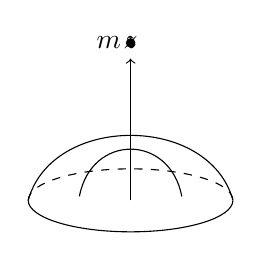
\begin{tikzpicture}[scale=1]
    \filldraw (0,2) circle (1.5pt) node[left] {$m$};
    \draw[->] (0,0) -- (0,1.8) node[above] {$z$};
    \draw (-1.3,0) arc (180:360:1.3 and 0.4);
    \draw[dashed] (-1.3,0) arc (180:0:1.3 and 0.4);
    \draw (-1.3,0) .. controls (-1.0,1.1) and (1.0,1.1) .. (1.3,0);
    \draw (-0.65,0.05) .. controls (-0.5,0.85) and (0.5,0.85) .. (0.65,0.05);
\end{tikzpicture}
\end{center}
$\Rightarrow$ invariância sob rotação na direção $\hat{z}$.

\textbf{3)} Partícula interagindo com uma esfera perfeita.
\begin{center}
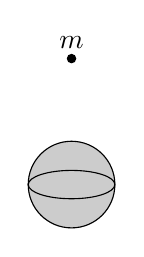
\begin{tikzpicture}[scale=1]
    \filldraw (0,1.6) circle (1.5pt) node[above] {$m$};
    \filldraw[gray!40] (0,0) circle (0.55);
    \draw (0,0) circle (0.55);
    \draw (0,0) ellipse (0.55 and 0.18);
\end{tikzpicture}
\end{center}
$\Rightarrow$ invariância sob rotação \textbf{EM QUALQUER EIXO}.

Nesse caso (3) temos $L_x(t), L_y(t)$ e $L_z(t) = \text{const}$ na MC, e $\langle L_x\rangle, \langle L_y\rangle, \langle L_z\rangle = \text{const}$ na MQ.

\subsection*{Invariância sob translação e conservação de momento linear}

De modo análogo podemos conectar invariância sob translação e conservação de momento linear.

\textbf{Mec. Clássica:}
\begin{equation}
    H(\vec{r}+a\hat{n}, \vec{p}) = H(\vec{r},\vec{p}) \qquad \forall\,a,\ \forall\,(\vec{r},\vec{p})
\label{eq:aula21_transl_mc_1}
\end{equation}

\begin{equation}
    \Longrightarrow \quad H(\vec{r}+\varepsilon\hat{n}, \vec{p}) = H(\vec{r},\vec{p})
\label{eq:aula21_transl_mc_2}
\end{equation}

\begin{equation}
    \Longrightarrow \quad H(\vec{r},\vec{p}) + \varepsilon\,\hat{n}\cdot\frac{\partial H}{\partial \vec{r}} + \dots = H(\vec{r},\vec{p})
\label{eq:aula21_transl_mc_3}
\end{equation}

\begin{equation}
    \Longrightarrow \quad \hat{n}\cdot\frac{\partial H}{\partial \vec{r}} = 0
    \quad \Longrightarrow \quad
    \boxed{\{H,\ \hat{n}\cdot\vec{p}\} = 0 \;\Longrightarrow\; \frac{d}{dt}(\hat{n}\cdot\vec{p}) = 0}
\label{eq:aula21_transl_mc_final}
\end{equation}

\textbf{Mec. Quântica:}
\begin{equation}
    \bra{\Psi} T^{\dagger}(a\hat{n})\, H\, T(a\hat{n}) \ket{\Psi} = \bra{\Psi} H \ket{\Psi} \qquad \forall\,a,\ \forall\,\ket{\Psi}
\label{eq:aula21_transl_mq_1}
\end{equation}

\begin{equation}
    \Longrightarrow \quad \bra{\Psi} T^{\dagger}(\varepsilon\hat{n})\, H\, T(\varepsilon\hat{n}) \ket{\Psi} = \bra{\Psi} H \ket{\Psi}
\label{eq:aula21_transl_mq_2}
\end{equation}

\begin{equation}
    \Longrightarrow \quad [H, T(\varepsilon\hat{n})] = 0
\label{eq:aula21_transl_mq_3}
\end{equation}

usando $T(\varepsilon\hat{n}) = \mathbb{I} - i\,\hat{n}\cdot\hat{P}\,\varepsilon/\hbar + \dots$
\begin{equation}
    \Longrightarrow \quad \boxed{[H,\ \hat{n}\cdot\vec{P}] = 0 \;\Longrightarrow\; \frac{d}{dt}\langle \hat{n}\cdot\vec{P} \rangle = 0}
\label{eq:aula21_transl_mq_final}
\end{equation}
